% !TeX program = xelatex
% Approved increment: textbook section 1.5; previous parts remain independent.
\documentclass[12pt,a4paper]{article}
\RequirePackage{array}[=2024-06-01]
% !TeX root = ../2/main.tex
\usepackage[a4paper,margin=25mm,headheight=16pt]{geometry}
\usepackage{amsmath,amssymb}
\usepackage{graphicx}
\usepackage{booktabs}
\usepackage{tabularx}
\usepackage{siunitx}
\usepackage{tikz}
\usepackage{circuitikz}
\usepackage[unicode,hidelinks]{hyperref}
\usepackage{xepersian}
% Only the regular B Nazanin file is installed; synthesize bold explicitly.
\settextfont[Path=C:/Windows/Fonts/,AutoFakeBold=2,AutoFakeSlant=0.2]{B-NAZANIN.TTF}
% B Nazanin lacks U+066A (Arabic percent), required by xepersian's digit setup.
% Arial covers the complete required digit/punctuation set; Persian prose remains B Nazanin.
\setdigitfont[Path=C:/Windows/Fonts/,BoldFont=arialbd.ttf,ItalicFont=ariali.ttf,BoldItalicFont=arialbi.ttf]{arial.ttf}
\setmathdigitfont[Path=C:/Windows/Fonts/,BoldFont=arialbd.ttf,ItalicFont=ariali.ttf,BoldItalicFont=arialbi.ttf]{arial.ttf}
\setlatintextfont{TeX Gyre Termes}
% B Nazanin does not contain the default itemize bullet and dash glyphs.
\renewcommand{\labelitemi}{\(\bullet\)}
\renewcommand{\labelitemii}{\(\circ\)}
\renewcommand{\labelitemiii}{\(\diamond\)}
\setlength{\parindent}{0pt}
\setlength{\parskip}{0.5em}
\linespread{1.25}
\newcommand{\exercise}[1]{\section*{تمرین #1}}
% !TeX root = ../2/main.tex
% Shared title page for every assignment.
% Change only \AssignmentNumber and \AssignmentDate in each main document.

\newcommand{\AssignmentNumber}[1]{\gdef\assignmentnumber{#1}}
\newcommand{\AssignmentDate}[1]{\gdef\assignmentdate{#1}}

\newcommand{\assignmentnumber}{---}
\newcommand{\assignmentdate}{---}

% Stable course metadata
\newcommand{\universityname}{دانشگاه صنعتی امیرکبیر}
\newcommand{\universityalias}{پلی‌تکنیک تهران}
\newcommand{\facultyname}{دانشکده مهندسی کامپیوتر}
\newcommand{\coursename}{طراحی مدارهای مجتمع پرتراکم پیشرفته}
\newcommand{\studentname}{محمد خلیلی اصل}
\newcommand{\instructorname}{دکتر مهدی صدیقی}

\newcommand{\MakeAssignmentCover}{%
  \begin{titlepage}
    \thispagestyle{empty}
    \centering
    \linespread{1}\selectfont

    \vspace*{0mm}
    
\includegraphics[width=44mm]{assets/aut-logo-black.png}\par
    \vspace{3mm}

    {\Large\bfseries \universityname\par}
    \vspace{1mm}
    {\large (\universityalias)\par}
    \vspace{1mm}
    {\large \facultyname\par}

    \vspace{8mm}
    {\Large\bfseries درس \coursename\par}

    \vspace{12mm}
    {\large عنوان\par}
    \vspace{2mm}
    {\LARGE\bfseries تمرین شماره \assignmentnumber\par}

    \vspace{10mm}
    {\large تهیه‌کننده\par}
    \vspace{2mm}
    {\Large\bfseries \studentname\par}

    \vspace{10mm}
    {\large استاد درس\par}
    \vspace{2mm}
    {\Large\bfseries \instructorname\par}

    \vspace{10mm}
    {\Large \assignmentdate\par}
    \vfill
  \end{titlepage}
  \setcounter{page}{1}%
}


\XeTeXgenerateactualtext=1
\newcommand{\secnum}[1]{\mbox{\beginL#1\endL}}
\setlength{\emergencystretch}{3em}
\AtBeginDocument{\DeclareSIPrefix{\micro}{\text{\lr{µ}}}{-6}}
\widowpenalty=10000
\clubpenalty=10000
\hypersetup{pdftitle={جزوه اول؛ Fabrication و Layout}}
\AssignmentNumber{جزوه اول؛ \lr{Fabrication} و \lr{Layout}}
\AssignmentDate{بخش \secnum{۱.۵} کتاب}
\patchcmd{\MakeAssignmentCover}{تمرین شماره \assignmentnumber}{\assignmentnumber}{}{\errmessage{Cover title replacement failed}}
\begin{document}
\MakeAssignmentCover
\section*{هدف و مرز این بخش}
در بخش قبلی، تابع منطقی را به شبکه ترانزیستور تبدیل کردیم.
اکنون می‌خواهیم بدانیم همین شبکه چگونه با ناحیه‌های مواد و اتصال‌ها ساخته و
در نمای بالا خوانده می‌شود. پیش‌نیاز این بخش، شناخت پایانه‌های \lr{MOS}،
عملکرد \lr{Inverter} و اتصال سری و موازی است؛ مفاهیم تازه ساخت و هندسه
در همین متن معرفی می‌شوند.

دامنه این فایل، تمام زیربخش‌های \secnum{۱.۵.۱} تا \secnum{۱.۵.۵} کتاب
\lr{Weste} و \lr{Harris} است \cite{weste}.
اسلایدهای محلی \lr{00} و \lr{01} زمینه ساختار ترانزیستور و گیت‌ها را فراهم کرده‌اند
\cite{intro,mos}؛ جزئیات ساخت، قواعد عددی و مثال‌های این بخش از خود کتاب گرفته شده‌اند.
شماره‌های بخش و شکل کتاب با شماره‌گذاری داخلی این جزوه متفاوت‌اند.

مدل فرایند این فصل، یک فرایند ساده آموزشی \lr{n-well CMOS} است؛
نباید آن را دستور ساخت کامل فناوری روز دانست.
شکل‌های توپولوژی ابعاد قابل ساخت را تضمین نمی‌کنند؛ شکل‌های اندازه‌دار نیز
فقط قواعد صریحاً ذکرشده در همین مدل را نشان می‌دهند.
در این گام، \lr{CAD}، \lr{Design Rule Checking (DRC)} یا
\lr{Layout Versus Schematic (LVS)} واقعی اجرا نشده است.

\tableofcontents
\clearpage
% !TeX root = booklet-01.tex
\section{از شماتیک تا مقطع و نمای بالا}
\label{sec:layout-views}
\subsection{سه نمایش از یک مدار}
شماتیک می‌گوید کدام پایانه‌ها به هم وصل‌اند؛ فاصله و اندازه خطوط آن عموماً معنای
ساخت ندارد. \lr{Layout} نمای بالای هندسه لایه‌هاست و محل و ابعاد اجزا را مشخص می‌کند.
\lr{Cross-section} برش عمودی از یک مسیر مشخص روی همان \lr{Layout} است؛
فقط اجزایی را نشان می‌دهد که صفحه برش از آن‌ها می‌گذرد
\cite[بخش \secnum{۱.۵} و شکل‌های \secnum{۱.۳۴} و \secnum{۱.۳۵}]{weste}.
پس ممکن است دو \lr{Gate} در شماتیک متصل باشند، ولی سیم مشترک آن‌ها در مقطع خاص دیده نشود.
برای فهم مدار باید اتصال‌های خارج از صفحه برش را نیز از نمای بالا یا برچسب‌ها خواند.

\lr{Layer} در نقشه، یک رده هندسه یا یک مرحله تعریف فرایند است.
هر رنگ لزوماً یک ورقه رسانای مجزا نیست؛ مثلاً \lr{n-well} ناحیه‌ای در خود
نیمه‌هادی و \lr{Contact} محل بازشدن عایق برای اتصال است.
دو مستطیل که از بالا هم‌پوشانی دارند، ممکن است در ارتفاع‌های متفاوت و عایق‌شده باشند.
این نکته در خواندن تقاطع \lr{Metal} و \lr{Poly} ضروری است.

\subsection{مقطع \lr{CMOS Inverter} و اتصال پایانه‌های آن}
در مثال کتاب، بستر \lr{p-substrate} است. \lr{nMOS} در همان بستر و
\lr{pMOS} در ناحیه \lr{n-well} ساخته می‌شود.
هر \lr{nMOS} دو ناحیه \(n^+\) و هر \lr{pMOS} دو ناحیه \(p^+\)
برای \lr{Source} و \lr{Drain} دارد.
علامت \(+\) شدت زیاد \lr{Doping} را نشان می‌دهد، نه بار مثبت ناحیه
\cite[بخش \secnum{۱.۵.۱}]{weste}.

در \lr{Inverter}، \lr{Source} ترانزیستور پایین به زمین، \lr{Source}
ترانزیستور بالا به تغذیه، دو \lr{Drain} به خروجی \(Y\) و دو \lr{Gate}
به ورودی \(A\) متصل‌اند. بدنه \lr{nMOS} باید مرجع پایین و بدنه \lr{pMOS}
مرجع بالا را بگیرد. شکل \ref{fig:layout-crosssection} این ساختار را به‌شکل ساده نشان می‌دهد.

\begin{figure}[ht]
\centering
\begin{latin}
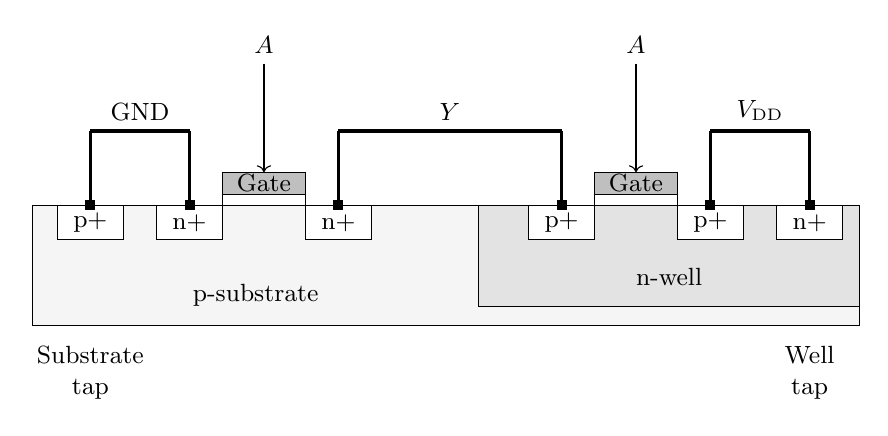
\begin{tikzpicture}[x=1.05cm,y=0.95cm,font=\small]
\draw[fill=gray!8] (0,0) rectangle (10,1.6);
\draw[fill=gray!22] (5.4,0.25) rectangle (10,1.6);
\node at (2.7,0.4) {p-substrate};\node at (7.7,0.65) {n-well};
\foreach \a/\b/\lab in {0.3/1.1/p+,1.5/2.3/n+,3.3/4.1/n+,6/6.8/p+,7.8/8.6/p+,9/9.8/n+} {
\draw[fill=white] (\a,1.15) rectangle (\b,1.6);
\node at ({(\a+\b)/2},1.37) {\lab};}
\foreach \a/\b in {2.3/3.3,6.8/7.8} {
\draw[fill=white] (\a,1.6) rectangle (\b,1.75);
\draw[fill=gray!50] (\a,1.75) rectangle (\b,2.05);}
\node at (2.8,1.9) {Gate};\node at (7.3,1.9) {Gate};
\foreach \x in {0.7,1.9,3.7,6.4,8.2,9.4} {
\draw[very thick] (\x,1.6)--(\x,2.6);
\fill (\x-0.06,1.55) rectangle (\x+0.06,1.68);}
\draw[very thick] (0.7,2.6)--(1.9,2.6) node[midway,above] {GND};
\draw[very thick] (3.7,2.6)--(6.4,2.6) node[midway,above] {$Y$};
\draw[very thick] (8.2,2.6)--(9.4,2.6) node[midway,above] {$V_{\mathrm{DD}}$};
\draw[->] (2.8,3.5) node[above] {$A$}--(2.8,2.05);
\draw[->] (7.3,3.5) node[above] {$A$}--(7.3,2.05);
\node[below,align=center] at (0.7,-0.15) {Substrate\\tap};
\node[below,align=center] at (9.4,-0.15) {Well\\tap};
\end{tikzpicture}
\end{latin}
\caption{طرح مفهومی مقطع \lr{Inverter} بر پایه شکل \secnum{۱.۳۴} کتاب \cite{weste}.
ابعاد و ارتفاع‌ها واقعی نیستند؛ خط‌های ضخیم اتصال رسانشی و مربع‌های کوچک محل تماس‌اند.
فضای بالای بستر، به‌جز محل تماس و رساناها، عایق فرض شده است.
دو \lr{Gate} با برچسب \(A\) در خارج از این برش به هم وصل می‌شوند.}
\label{fig:layout-crosssection}
\end{figure}

\subsection{چرا \lr{Tap} لازم است؟}
\lr{Substrate Tap} یک ناحیه \(p^+\) در بستر \lr{p} و \lr{Well Tap}
یک ناحیه \(n^+\) داخل چاه \lr{n} است. تماس فلزی با این ناحیه‌های پرناخالصی،
اتصال کم‌مقاومت به بدنه را فراهم می‌کند.
تماس با نیمه‌هادی کم‌ناخالصی می‌تواند رفتار \lr{Schottky} و یکسوساز داشته باشد؛
\lr{Doping} زیاد برای تماس \lr{Ohmic} مناسب است
\cite[صفحه چاپی ۲۰]{weste}.

اتصال بستر به زمین و چاه به تغذیه، در محدوده معمول ولتاژهای مدار، از
بایاس مستقیم ناخواسته پیوندهای بدنه با \lr{Source/Drain} جلوگیری می‌کند.
\textbf{تماس \lr{Source} جای \lr{Tap} بدنه را نمی‌گیرد.}
در \lr{nMOS}، ناحیه \(n^+\) مربوط به \lr{Source} و ناحیه \(p^+\)
مربوط به بدنه، دو ناحیه متفاوت‌اند؛ حتی اگر هر دو با فلز به زمین متصل شوند.
به همین ترتیب \lr{pMOS} برای بدنه \lr{n-well} به تماس \(n^+\) نیاز دارد.

\subsection{نقش عایق نازک، عایق میدان و تماس}
\lr{Gate Oxide} لایه نازک میان \lr{Gate} و کانال است؛ میدان را منتقل
می‌کند، ولی در مدل ایدئال مسیر رسانشی مستقیم نیست.
\lr{Field Oxide} و عایق‌های بین لایه‌ها، ناحیه‌ها و فلز را از مسیرهای
ناخواسته جدا می‌کنند. سوراخ \lr{Contact} فقط در محل مجاز، اتصال فلز به
\lr{Diffusion} یا \lr{Poly} را برقرار می‌کند.
اتصال میان دو لایه فلزی را معمولاً \lr{Via} می‌نامیم.
پس روی هم افتادن \lr{Metal1} و \lr{Poly} بدون \lr{Contact}، آن‌ها را اتصال کوتاه نمی‌کند.

در مدل ساده این فصل، \lr{Poly} روی ناحیه فعال از عایق نازک جدا می‌شود و
ترانزیستور را می‌سازد. این تقاطع نیز اتصال کوتاه \lr{Gate} به کانال نیست.
تفاوت میان «تماس»، «تقاطع ترانزیستوری» و «عبور عایق‌شده» را در همه شکل‌ها حفظ می‌کنیم.

\section{مراحل آموزشی \lr{Fabrication}}
\label{sec:layout-fabrication}
\subsection{ماسک چیست و چرا شش ماسک کافیِ واقعی نیست؟}
\lr{Mask} الگوی هندسی انتخاب ناحیه‌ها در یک مرحله فرایند است.
کتاب برای توضیح \lr{Inverter} از مجموعه فرضی شش ماسک شامل
\lr{n-well}، \lr{Polysilicon}، \lr{n-diffusion}، \lr{p-diffusion}،
\lr{Contact} و \lr{Metal} استفاده می‌کند
\cite[بخش \secnum{۱.۵.۲} و شکل \secnum{۱.۳۵}]{weste}.
این شش نام، مراحل کامل یک فرایند صنعتی نیستند.
به‌ویژه هندسه‌های نهایی \lr{Layout} لزوماً با ماسک‌های واقعیِ بیشتر و اصلاح‌شده،
رابطه یک‌به‌یک ندارند.

\lr{Photolithography} با استفاده از نور و \lr{Photoresist}، الگوی ماسک
را روی لایه‌ای حساس منتقل می‌کند. \lr{Etching} ماده را از ناحیه‌های بازشده
برمی‌دارد. \lr{Deposition} ماده اضافه می‌کند و \lr{Oxidation} لایه اکسید را
با واکنش روی سطح ایجاد می‌کند. \lr{Doping} نوع و غلظت حامل‌ها را در ناحیه انتخاب‌شده تغییر می‌دهد.
این عمل‌ها نقش یکسان ندارند؛ برداشتن \lr{Photoresist} به معنی حذف چاه یا رسانای زیر آن نیست.

\subsection{ساخت \lr{n-well}: الگوگذاری را مرحله‌به‌مرحله دنبال کنیم}
شکل \secnum{۱.۳۶} کتاب، ساخت چاه را در چند مقطع نشان می‌دهد. ترتیب آموزشی آن چنین است
\cite[صفحات چاپی ۲۱ تا ۲۳]{weste}:
\begin{enumerate}
\item از ویفر \lr{p-type} آغاز می‌کنیم. کل ویفر، یک تراشه منفرد نیست؛
ناحیه‌های چندین تراشه روی آن پردازش می‌شوند.
\item یک اکسید محافظ روی سطح تشکیل می‌شود. در مثال کتاب، رشد حرارتی اکسید
با واکنش \lr{Si} و اکسیژن انجام می‌شود؛ این لایه در این مرحله سد انتخاب ناحیه است.
\item سطح با \lr{Photoresist} پوشانده و از پشت ماسک چاه نوردهی می‌شود.
کتاب نوعی رفتار مثبت را توصیف می‌کند: بخش نورخورده در مرحله \lr{Develop} حذف می‌شود.
این قرارداد را نباید بی‌قید به همه انواع \lr{Resist} تعمیم داد.
\item در ناحیه باز \lr{Resist}، اکسید \lr{Etch} می‌شود؛ اکسید زیر بخش
محافظت‌شده باقی می‌ماند. پس اکنون سوراخی در سد اکسیدی داریم.
\item \lr{Resist} باقی‌مانده پاک می‌شود؛ ماسک اکسیدی هنوز روی ویفر وجود دارد.
این تمایز لازم است، چون مرحله ورود ناخالصی باید همچنان انتخابی باشد.
\item ناخالصی مناسب \lr{n-type} در ناحیه باز وارد می‌شود تا نوع آن بخش
از بستر تغییر کند و چاه تشکیل شود. انتشار جانبی می‌تواند مرز نهایی را
با لبه هندسی سوراخ یکسان نگه ندارد.
\item اکسید محافظ باقی‌مانده پاک می‌شود؛ چاه که داخل نیمه‌هادی تشکیل شده،
با برداشتن اکسید از بین نمی‌رود.
\end{enumerate}

شکل \ref{fig:layout-well-stages} سه مقطع از همین مسیر را کنار هم می‌گذارد.
در مقطع میانی، \lr{Resist} برداشته شده ولی سد اکسیدی باقی است؛
با مقطع نهایی که اکسید محافظ حذف شده تفاوت دارد.
\begin{figure}[ht]
\centering
\begin{latin}
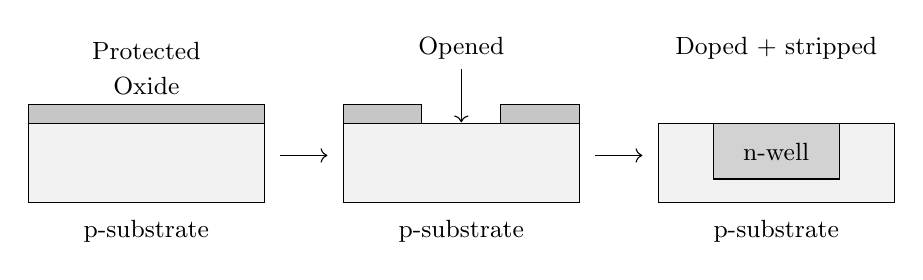
\begin{tikzpicture}[x=1cm,y=1cm,font=\small]
\foreach \shift/\lab in {0/Protected,4/Opened,8/{Doped + stripped}} {
\begin{scope}[xshift=\shift cm]
\draw[fill=gray!10] (0,0) rectangle (3,1);
\node[above] at (1.5,1.7) {\lab};
\node[below] at (1.5,-0.1) {p-substrate};
\end{scope}}
\draw[fill=gray!45] (0,1) rectangle (3,1.25);
\node[above] at (1.5,1.25) {Oxide};
\draw[fill=gray!45] (4,1) rectangle (5,1.25);
\draw[fill=gray!45] (6,1) rectangle (7,1.25);
\draw[->] (5.5,1.7)--(5.5,1.02);
\draw[fill=gray!35] (8.7,0.3) rectangle (10.3,1);
\node at (9.5,0.65) {n-well};
\draw[->] (3.2,0.6)--(3.8,0.6);
\draw[->] (7.2,0.6)--(7.8,0.6);
\end{tikzpicture}
\end{latin}
\caption{سه وضعیت انتخاب‌شده از ساخت چاه، بر پایه شکل \secnum{۱.۳۶} کتاب
\cite{weste}؛ همه مراحل \lr{Lithography} در این تصویر فشرده رسم نشده‌اند.
پهن‌تر بودن چاه از پنجره، اثر مفهومی انتشار جانبی است؛ اندازه‌ها واقعی نیستند.}
\label{fig:layout-well-stages}
\end{figure}

\lr{Diffusion} یعنی حرکت اتم‌های ناخالصی در ماده در شرایط مناسب حرارتی.
در \lr{Ion Implantation}، یون‌ها با میدان شتاب می‌گیرند و به سطح وارد می‌شوند.
کتاب هر دو را برای افزودن ناخالصی توضیح می‌دهد؛ نتیجه و پروفایل واقعی آن‌ها
به فرایند وابسته است. از نام ماسک \lr{Diffusion} نباید نتیجه گرفت تمام
ناحیه‌های موسوم به \lr{Diffusion} الزاماً با همان روش قدیمی ساخته شده‌اند.

\subsection{ساخت \lr{Gate} و معنای \lr{Self-aligned}}
پس از چاه، اکسید نازک \lr{Gate} و لایه \lr{Polysilicon} تشکیل می‌شوند.
در فرایند توضیحی کتاب، \lr{Chemical Vapor Deposition (CVD)} برای تشکیل
\lr{Poly} به کار می‌رود و ناخالصی مناسب رسانایی آن را افزایش می‌دهد.
با ماسک \lr{Poly}، فقط نوارهای موردنیاز باقی می‌مانند
\cite[شکل \secnum{۱.۳۷}]{weste}.

سپس انتخاب ناحیه‌های \(n^+\) برای \lr{nMOS} و تماس چاه انجام می‌شود.
\lr{Gate} موجود، ورود ناخالصی را در محل کانال مسدود می‌کند؛
بنابراین دو ناحیه \lr{Source} و \lr{Drain} در دو سوی همان \lr{Gate}
تشکیل می‌شوند. این \lr{Self-aligned Gate} به معنی خودترازی لبه‌های مرتبط با
\lr{Gate} است، نه بی‌نیازی کل تراشه از هم‌ترازی ماسک‌ها.

برای ناحیه‌های \(p^+\)، انتخاب نوع مخالف تکرار می‌شود تا \lr{Source/Drain}
ترانزیستور \lr{pMOS} و تماس بستر ساخته شوند.
ناحیه فعال \lr{nMOS} باید در بستر \lr{p} و ناحیه فعال \lr{pMOS} داخل چاه
\lr{n} قرار گیرد. فقط عوض کردن رنگ یا برچسب نقشه، این شرط فیزیکی را تامین نمی‌کند.

\subsection{عایق، \lr{Contact} و اتصال فلزی}
در مدل کتاب، عایق میان فلز و ناحیه‌های زیرین قرار می‌گیرد؛ ماسک \lr{Contact}
جاهایی را باز می‌کند که اتصال لازم است. سپس فلز نشانده و با ماسک خودش الگوگذاری می‌شود.
در مثال ساده، آلومینیوم و فرایند \lr{Sputtering} توصیف شده‌اند؛
این انتخاب مواد، مشخصه همان مدل توضیحی است، نه الزام همه فرایندها
\cite[شکل \secnum{۱.۳۸}]{weste}.

اگر چند لایه فلزی داشته باشیم، عایق، الگوگذاری فلز و اتصال‌های بین لایه‌ای
نیز لازم می‌شوند. شمار ماسک‌های واقعی و روش عایق‌سازی و متالیزاسیون می‌تواند
بسیار پیچیده‌تر باشد. در این بخش، هدف دنبال کردن نقش لایه‌هاست؛
نه ارائه دستور اجرایی آزمایشگاه ساخت.

\subsection{چرا مساحت مهم است؟}
بخش زیادی از مراحل روی ویفر و تعداد زیادی تراشه تکرار می‌شود؛
ازاین‌رو مساحت هر تراشه بر تعداد تراشه‌های قابل جاگذاری اثر دارد.
در یک برآورد هندسی، کاهش مساحت \(A\) در مساحت قابل‌استفاده ثابت ویفر
\(A_{\mathrm{wafer}}\)، تعداد خام را تقریباً به نسبت
\(A_{\mathrm{wafer}}/A\) افزایش می‌دهد.
این نسبت، برش لبه، خطوط جداسازی و \lr{Yield} را لحاظ نمی‌کند؛
پس هزینه دقیق تراشه فقط با شمار ترانزیستور یا این نسبت تعیین نمی‌شود.
این توضیح، برداشت ساده بخش \secnum{۱.۵.۲} کتاب از اهمیت مساحت را با فرض‌هایش روشن می‌کند.

\subsection{پرسش‌های ساخت با پاسخ}
\begin{enumerate}
\item \textbf{پس از پاک کردن ماسک اکسیدی، چرا چاه باقی می‌ماند؟}
چاه ناحیه‌ای با ناخالصی تغییرکرده داخل نیمه‌هادی است؛ اکسید پوشش انتخابی روی سطح بود.
\item \textbf{آیا \lr{Gate} با کانال تماس رسانشی مستقیم دارد؟}
در مدل ایدئال خیر؛ عایق نازک میان آن‌هاست. تقاطع در نمای بالا به معنی اتصال کوتاه نیست.
\item \textbf{چرا تماس بدنه \lr{pMOS} از نوع \(n^+\) است؟}
چون به بدنه \lr{n-well} وصل می‌شود؛ ناحیه‌های \(p^+\) آن ترانزیستور مربوط به \lr{Source/Drain} هستند.
\item \textbf{آیا شش ماسک معرفی‌شده تعداد ماسک‌های یک فناوری واقعی است؟}
خیر؛ این مجموعه برای توضیح مدار و مسیر ساخت فرض شده است و مراحل صنعتی بیشتری لازم است.
\end{enumerate}

% !TeX root = booklet-01.tex
\section{قواعد هندسی \lr{Layout}}
\label{sec:layout-rules}
\subsection{عرض، فاصله و پوشش را جدا کنیم}
\lr{Minimum Width} حداقل عرض یک ناحیه است؛ عرض خیلی کم می‌تواند ساخت
رسانای پیوسته را نامطمئن کند.
\lr{Minimum Spacing} فاصله لبه‌به‌لبه دو شکل است؛ فاصله کم خطر اتصال
ناخواسته یا نقض محدودیت‌های ساخت را ایجاد می‌کند.
\lr{Enclosure} مقدار پوشش لایه پیرامون شکل لایه دیگر، مثلاً فلز پیرامون
\lr{Contact} است؛ \lr{Overlap/Extension} امتداد لازم یک شکل از لبه شکل دیگر را بیان می‌کند.
این‌ها نقش‌های متفاوتی دارند و با فاصله مرکزبه‌مرکز یکسان نیستند
\cite[بخش \secnum{۱.۵.۳}]{weste}.

در شکل \ref{fig:layout-spacing}، دو خط با عرض \(w\) و فاصله آزاد \(s\)
داریم. فاصله مرکز دو خط برابر \(p=w+s\) است و \lr{Pitch} نامیده می‌شود.
اگر عرض‌ها متفاوت باشند، فاصله مرکزها \(w_1/2+s+w_2/2\) خواهد بود.

\begin{figure}[ht]
\centering
\begin{latin}
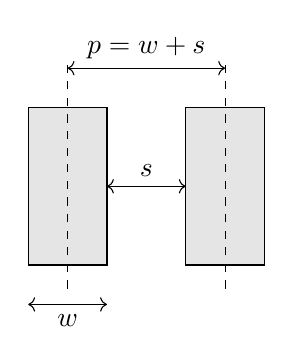
\begin{tikzpicture}[x=1cm,y=1cm]
\draw[fill=gray!20] (0,0) rectangle (1,2);
\draw[fill=gray!20] (2,0) rectangle (3,2);
\draw[dashed] (0.5,-0.3)--(0.5,2.6) (2.5,-0.3)--(2.5,2.6);
\draw[<->] (0,-0.5)--node[below] {$w$}(1,-0.5);
\draw[<->] (1,1)--node[above] {$s$}(2,1);
\draw[<->] (0.5,2.5)--node[above] {$p=w+s$}(2.5,2.5);
\end{tikzpicture}
\end{latin}
\caption{نمای آموزشی عرض، فاصله آزاد و \lr{Pitch}؛ خط‌چین‌ها محور میانی دو خط‌اند.}
\label{fig:layout-spacing}
\end{figure}

\subsection{معنای پارامتر \texorpdfstring{\(\lambda\)}{lambda}}
در قواعد مقیاس‌پذیر آموزشی، طول‌ها به صورت ضریبی از \(\lambda\) نوشته می‌شوند.
در قرارداد این فصل، حداقل طول ترانزیستور رسم‌شده معمولاً \(L_{\min}=2\lambda\)
است. بنابراین انتخاب \(\lambda\) مقیاس فیزیکی نقشه را تعیین می‌کند
\cite[صفحات چاپی ۲۴ و ۲۵]{weste}.
\(\lambda\) در اینجا واحد طول قراردادی است و نباید آن را با ضریب
\lr{Channel Length Modulation} که ممکن است همین حرف را داشته باشد اشتباه گرفت.

\textbf{مثال آموزشی تبدیل مقیاس.} اگر برای مدلی
\(L_{\min}=\qty{0.6}{\micro\metre}\) انتخاب شود، داریم:
\begin{equation}\label{eq:layout-lambda}
\lambda=\frac{L_{\min}}{2}=\qty{0.3}{\micro\metre},\qquad
4\lambda=\qty{1.2}{\micro\metre}.
\end{equation}
ابتدا مقدار فیزیکی یک \(\lambda\) را یافتیم؛ سپس در ضریب هندسی ضرب کردیم.
برای نمونه تاریخی حداقل طول \(\qty{180}{\nano\metre}\)، قرارداد ساده
\(\lambda=\qty{90}{\nano\metre}\) می‌دهد. کتاب در پانوشت توضیح می‌دهد
که حتی برای فرایندهای هم‌نام نیز قرارداد دقیق می‌تواند متفاوت باشد.

این مدل برای یادگیری هندسه و مقیاس مفید است؛ همه قواعد واقعی با یک ضریب
یکسان کوچک نمی‌شوند. نام یک \lr{Technology Node} نیز به‌تنهایی
جدول قابل‌اعمال \lr{Design Rules} را مشخص نمی‌کند.
برای ساخت واقعی باید قواعد و لایه‌های همان \lr{Process Design Kit (PDK)} به کار روند؛
در این جزوه از \lr{PDK} خاصی استفاده نشده است.

\subsection{قواعد ساده کتاب و دامنه کاربردشان}
جدول \ref{tab:layout-rules} خلاصه قواعد ساده و محافظه‌کارانه کتاب برای
مدل \lr{n-well} با دو لایه فلزی است
\cite[صفحات چاپی ۲۵ و ۲۶، شکل \secnum{۱.۳۹}]{weste}.
این جدول تمام قواعد یک فرایند نیست و به معنای تایید ساخت یک \lr{Layout} کامل نیست.

\begin{table}[ht]
\centering
\caption{قواعد آموزشی مبتنی بر \(\lambda\)، برگرفته از کتاب؛ همه اعداد ضرایب \(\lambda\) هستند.}
\label{tab:layout-rules}
\begin{tabularx}{\textwidth}{Xc}
\toprule
ویژگی & مقدار\\
\midrule
حداقل عرض و فاصله آزاد فلز و \lr{Diffusion} & \(4\lambda\)\\
اندازه \lr{Contact} & \(2\lambda\times2\lambda\)\\
پوشش لازم اطراف \lr{Contact} در لایه‌های بالا و پایین & \(1\lambda\)\\
عرض \lr{Poly} & \(2\lambda\)\\
امتداد \lr{Poly} از مرز \lr{Diffusion} در محل ترانزیستور & \(2\lambda\)\\
فاصله \lr{Poly} از \lr{Diffusion} در محل بدون ترانزیستور & \(1\lambda\)\\
فاصله آزاد \lr{Poly}ها و فاصله تماس از \lr{Poly} یا تماس دیگر & \(3\lambda\)\\
پوشش چاه پیرامون \lr{pMOS} و فاصله چاه از \lr{nMOS} & \(6\lambda\)\\
\bottomrule
\end{tabularx}
\end{table}

برای ترانزیستور، \lr{Poly} باید ناحیه فعال را کامل قطع کند و از دو لبه آن
به‌اندازه لازم بیرون بزند؛ این امتداد جلوی باقی‌ماندن مسیر ناخواسته دور \lr{Gate}
را می‌گیرد. اگر ترانزیستور نمی‌خواهیم، باید فاصله آزاد را حفظ کنیم؛
تقاطع تصادفی \lr{Poly} و \lr{Active} می‌تواند قطعه ناخواسته بسازد.

\lr{Contact} باید از هر طرف با لایه‌های مجاز پوشانده شود؛ صرف قرار گرفتن
مرکز آن داخل فلز کافی نیست. از جدول می‌توان حداقل عرض ناحیه تماس‌پذیر را استخراج کرد:
\begin{equation}\label{eq:layout-contact}
w_{\mathrm{landing}}=1\lambda+2\lambda+1\lambda=4\lambda.
\end{equation}
شکل \ref{fig:layout-contact} این محاسبه را برای یک بعد نشان می‌دهد؛
در بعد دیگر نیز همین پوشش لازم است.

\begin{figure}[ht]
\centering
\begin{latin}
% Dimension values remain Persian even in the Latin diagram environment.
\PersianMathDigits
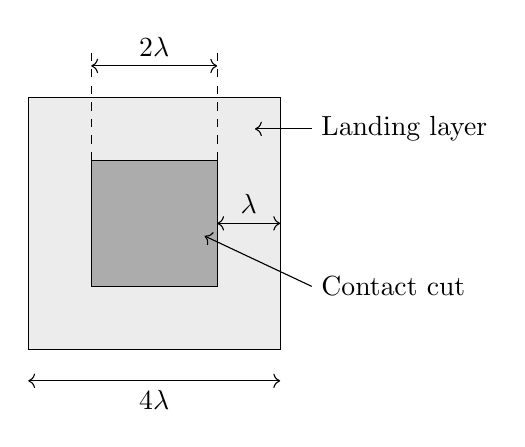
\begin{tikzpicture}[x=0.8cm,y=0.8cm]
\draw[fill=gray!15] (0,0) rectangle (4,4);
\draw[fill=gray!65] (1,1) rectangle (3,3);
\draw[<->] (0,-0.5)--node[below] {$4\lambda$}(4,-0.5);
\draw[<->] (1,4.5)--node[above] {$2\lambda$}(3,4.5);
\draw[dashed] (1,3)--(1,4.7) (3,3)--(3,4.7);
\draw[<->] (3,2)--node[above] {$\lambda$}(4,2);
\node[right] at (4.5,3.5) {Landing layer};
\draw[->] (4.5,3.5)--(3.6,3.5);
\node[right] at (4.5,1) {Contact cut};\draw[->] (4.5,1)--(2.8,1.8);
\end{tikzpicture}
\end{latin}
\caption{مثال اندازه‌دار برای رابطه \eqref{eq:layout-contact}.
مربع داخلی، محل برش تماس و مربع بیرونی، مرز حداقل لایه پوشاننده است؛
لایه دیگر اتصال نیز باید پوشش و قواعد مستقل خود را داشته باشد.}
\label{fig:layout-contact}
\end{figure}

اگر دو تماس \(2\lambda\) در امتداد عرض کنار هم و با فاصله آزاد
\(3\lambda\) قرار گیرند و در دو طرف \(1\lambda\) پوشش داشته باشند،
طول ناحیه لازم \((1+2+3+2+1)\lambda=9\lambda\) می‌شود.
این استدلال، مقدار ذکرشده در پانوشت کتاب برای تماس دوگانه را روشن می‌کند؛
دو تماس می‌توانند افزونگی اتصال را بهتر کنند، ولی صحت همه قواعد فرایند را تضمین نمی‌کنند.

\subsection{طول و عرض ترانزیستور را از کدام جهت بخوانیم؟}
طول کانال \(L\)، فاصله مسیر جریان زیر \lr{Gate} میان دو سوی
\lr{Source/Drain} است. عرض کانال \(W\)، اندازه عمود بر این مسیر در ناحیه
\lr{Gate} روی \lr{Active} است.
پس اگر \lr{Active} افقی و \lr{Poly} عمودی باشد، عرض افقی نوار \lr{Poly}
طول کانال و ارتفاع نوار \lr{Active} عرض کانال را تعیین می‌کند؛
شکل \ref{fig:layout-wl} برای همین جهت رسم شده است.

\begin{figure}[ht]
\centering
\begin{latin}
\PersianMathDigits
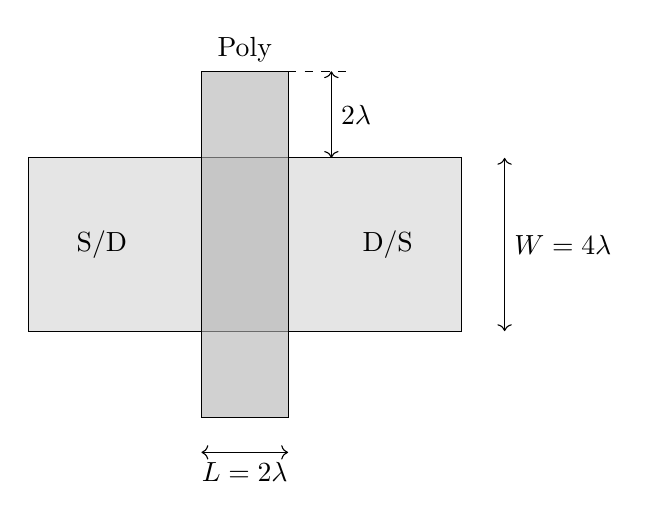
\begin{tikzpicture}[x=0.55cm,y=0.55cm]
\draw[fill=gray!20] (0,0) rectangle (10,4);
\draw[fill=gray!60,fill opacity=0.6] (4,-2) rectangle (6,6);
\node at (1.7,2) {S/D};\node at (8.3,2) {D/S};
\node[above] at (5,6) {Poly};
\draw[<->] (4,-2.8)--node[below] {$L=2\lambda$}(6,-2.8);
\draw[<->] (11,0)--node[right] {$W=4\lambda$}(11,4);
\draw[<->] (7,4)--node[right] {$2\lambda$}(7,6);
\draw[dashed] (6,4)--(7.5,4) (6,6)--(7.5,6);
\end{tikzpicture}
\end{latin}
\caption{طرح هندسی آموزشی یک کانال با \(W=4\lambda\) و \(L=2\lambda\).
امتداد \lr{Poly} از ناحیه فعال نیز نشان داده شده است؛ تماس‌های \lr{Source/Drain}
در این شکل حذف شده‌اند و شکل، \lr{Layout} کامل تماس‌دار نیست.}
\label{fig:layout-wl}
\end{figure}

نماد \(W/L=4/2\) در شکل‌های آموزشی کتاب یعنی \(W=4\lambda\) و
\(L=2\lambda\)، نه فقط نسبت عددی ۲ بدون مشخص بودن ابعاد.
ترانزیستورهای \(4/2\) و \(8/4\) نسبت یکسان دارند، ولی هندسه و ظرفیت‌هایشان
یکسان نیست. در مدل نمونه رابطه \eqref{eq:layout-lambda}،
\(4/2\) به \(\qty{1.2}{\micro\metre}/\qty{0.6}{\micro\metre}\) تبدیل می‌شود.

کتاب یک \lr{Unit Inverter} با \lr{nMOS} به ابعاد \(4/2\) و \lr{pMOS}
به ابعاد \(8/2\) نشان می‌دهد. حفره‌ها در مدل مورد بحث \lr{Mobility}
کمتری دارند؛ افزایش عرض \lr{pMOS} می‌تواند این تفاوت جریان را تا حدی جبران کند.
ضریب دو در این شکل یک انتخاب آموزشی است؛ قانون ثابت همه فناوری‌ها یا شرط لازم
برای درست بودن جدول منطقی \lr{Inverter} نیست
\cite[شکل \secnum{۱.۴۰}]{weste}.

\subsection{مثال‌های عددی و کنترل مستقل قواعد}
\begin{enumerate}
\item \textbf{دو خط فلزی با عرض \(4\lambda\) و فاصله محور \(7\lambda\):}
فاصله آزاد \(7\lambda-4\lambda=3\lambda\) است؛
قاعده \(4\lambda\) فاصله آزاد نقض شده است، حتی اگر عرض هر دو درست باشد.
\item \textbf{تماس \(2\lambda\) در ناحیه متقارن \(3\lambda\):}
پوشش هر طرف \((3-2)\lambda/2=0.5\lambda\) است؛
از \(1\lambda\) لازم کمتر است و کافی نیست.
\item \textbf{دو خط با عرض و فاصله \(4\lambda\):}
\lr{Pitch} برابر \(8\lambda\) است؛ با \(\lambda=\qty{0.3}{\micro\metre}\)
به \(\qty{2.4}{\micro\metre}\) تبدیل می‌شود.
\end{enumerate}
این کنترل‌ها فقط همان شرط محلی را می‌آزمایند؛ تایید عرض یک خط به معنی
تایید فاصله چاه، نوع تماس، اتصال مدار یا کل \lr{DRC} نیست.

% !TeX root = booklet-01.tex
\section{خواندن و ساخت توپولوژی گیت‌ها}
\label{sec:layout-gates}
\subsection{قرارداد لایه‌ها و تقاطع‌ها}
در این بخش، \lr{Active/Diffusion} ناحیه محل \lr{Source/Drain} و کانال است؛
نوع \(n\) یا \(p\) و چاه، نوع ترانزیستور را مشخص می‌کند.
\lr{Poly} در محل عبور از \lr{Active}، \lr{Gate} را می‌سازد.
\lr{Metal1} برای اتصال‌ها به کار می‌رود و مربع سیاه محل \lr{Contact} است.
چون شکل‌ها باید در چاپ سیاه‌وسفید هم خوانا باشند، برچسب و نوع خط در کنار تیرگی‌ها آمده است.

سه قاعده خواندن را روی شکل‌ها به کار ببرید:
\begin{enumerate}
\item دو شکل پیوسته از یک لایه رسانا، اتصال دارند؛ برای مثال دو بخش
\lr{Metal1} که به هم می‌رسند یک شبکه می‌سازند.
\item هم‌پوشانی دو لایه رسانای متفاوت، بدون \lr{Contact/Via} لزوماً اتصال نیست.
در این مدل، فلز عبوری از روی \lr{Poly} بدون تماس، از آن عایق است.
\item تقاطع \lr{Poly} با \lr{Active} یک ترانزیستور می‌سازد، نه اتصال مستقیم
\lr{Gate} به \lr{Source/Drain}. برای استخراج مدار، \lr{Active} را در محل
همین کانال‌ها به ناحیه‌های پایانه‌ای تقسیم می‌کنیم.
\end{enumerate}
این روش، پیوند نمای بالا و شماتیک در شکل‌های بخش \secnum{۱.۵.۴} کتاب را روشن می‌کند
\cite{weste}.

\subsection{سبک چهار نوار و \lr{Inverter}}
کتاب یک سبک ساده مناسب سلول را معرفی می‌کند: ریل زمین پایین، نوار
\lr{n-diffusion}، نوار \lr{p-diffusion} و ریل تغذیه بالا.
\lr{Poly}ها عمدتاً عمودی‌اند و فلز، پایانه‌های لازم را به هم وصل می‌کند.
این نظم، کنارهم‌گذاری سلول‌ها و دسترسی به پایه‌ها را آسان می‌کند؛
تنها سبک ممکن \lr{Layout} نیست
\cite[بخش \secnum{۱.۵.۴}]{weste}.
شکل \ref{fig:layout-inverter} نمونه توپولوژی \lr{Inverter} را با تماس‌های بدنه نشان می‌دهد.

\begin{figure}[ht]
\centering
\begin{latin}
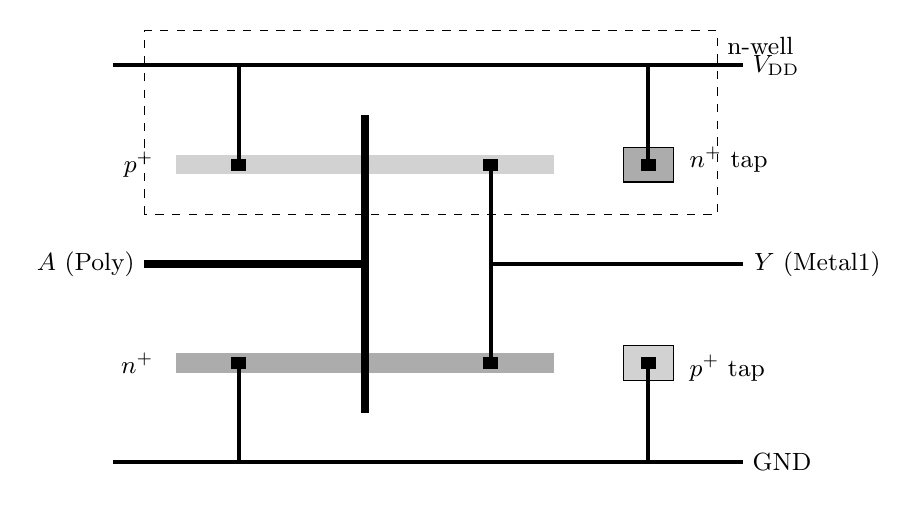
\begin{tikzpicture}[x=0.8cm,y=0.63cm,font=\small]
\draw[dashed] (0.5,5) rectangle (9.6,8.7);
\node[right] at (9.6,8.4) {n-well};
\draw[line width=7pt,gray!35] (1,6)--(7,6);
\draw[line width=7pt,gray!65] (1,2)--(7,2);
\node[left] at (0.8,6) {$p^+$};\node[left] at (0.8,2) {$n^+$};
\draw[line width=3pt] (4,1)--(4,7);
\draw[line width=3pt] (0.5,4)--(4,4);\node[left] at (0.5,4) {$A$ (Poly)};
\draw[line width=1.5pt] (0,8)--(10,8) (0,0)--(10,0);
\node[right] at (10,8) {$V_{\mathrm{DD}}$};\node[right] at (10,0) {GND};
\draw[line width=1.5pt] (2,6)--(2,8) (2,2)--(2,0);
\draw[line width=1.5pt] (6,6)--(6,2);
\draw[line width=1.5pt] (6,4)--(10,4) node[right] {$Y$ (Metal1)};
\draw[fill=gray!65] (8.1,5.65) rectangle (8.9,6.35);
\draw[fill=gray!35] (8.1,1.65) rectangle (8.9,2.35);
\draw[line width=1.5pt] (8.5,6)--(8.5,8) (8.5,2)--(8.5,0);
\foreach \x/\y in {2/6,6/6,2/2,6/2,8.5/6,8.5/2} {
\fill (\x-0.12,\y-0.12) rectangle (\x+0.12,\y+0.12);}
\node[right,align=left] at (9,6.1) {$n^+$ tap};
\node[right,align=left] at (9,1.9) {$p^+$ tap};
\end{tikzpicture}
\end{latin}
\caption{نمای بالای مفهومی \lr{Inverter} بر پایه شکل‌های \secnum{۱.۴۱}
و \secnum{۱.۳۵} کتاب \cite{weste}.
نوار خاکستری بالا \(p^+\)، پایین \(n^+\)، خط عمودی ضخیم وسط \lr{Poly}
و خط‌های نازک سیاه \lr{Metal1} هستند. ابعاد به مقیاس قواعد رسم نشده‌اند؛
این شکل توپولوژی است و ادعای عبور از \lr{DRC} ندارد.}
\label{fig:layout-inverter}
\end{figure}

در نوار پایین، تقاطع \lr{Poly} با \(n^+\) یک \lr{nMOS} می‌سازد؛
سمت چپ از تماس به زمین و سمت راست به خروجی می‌رود.
در نوار بالا یک \lr{pMOS} ساخته می‌شود؛ چپ آن به تغذیه و راست آن به همان خروجی وصل است.
ورودی، نوار \lr{Poly} مشترک است.
تماس‌های جداگانه سمت راست، بدنه‌ها را به ریل مربوط می‌رسانند؛
دو تماس خروجی و دو تماس بدنه یکی نیستند.

برای استخراج شماتیک، ابتدا دو تقاطع ترانزیستوری را بشمارید؛ سپس شبکه‌های فلزی
و تماس‌هایشان را دنبال کنید. نتیجه باید دقیقاً همان دو ترانزیستور با
\lr{Gate} مشترک و \lr{Drain} مشترک باشد.
اگر تماس خروجی یکی حذف شود، دیگر آن اتصال رسانشی در مدل نقشه برقرار نیست؛
اگر تماس ناخواسته روی محل نامناسب اضافه شود، ممکن است شبکه‌های مستقل اتصال کوتاه شوند.

\subsection{اشتراک \lr{Diffusion} و گیت \lr{NAND} سه‌ورودی}
سه \lr{Poly} با ورودی‌های \(A,B,C\) یک نوار \lr{n-diffusion} را قطع می‌کنند.
چهار ناحیه میان دو انتها و سه \lr{Gate} داریم: از سمت خروجی به زمین،
\(Y,x_1,x_2,GND\). کانال‌های میان آن‌ها به‌ترتیب با \(A,B,C\) کنترل می‌شوند.
گره‌های \(x_1,x_2\) داخلی‌اند و برای اتصال سری نیازی به تماس فلزی جدا ندارند؛
ناحیه مشترک، پایانه دو ترانزیستور مجاور را می‌سازد.

همان سه خط \lr{Poly}، نوار \lr{p-diffusion} را نیز قطع می‌کنند.
اگر فقط دو انتهای این نوار را سیم‌کشی کنیم، سه \lr{pMOS} سری خواهیم داشت؛
این برای \lr{NAND} درست نیست. باید چهار ناحیه بالایی را با فلز به‌ترتیب
به \(V_{\mathrm{DD}},Y,V_{\mathrm{DD}},Y\) وصل کنیم.
در نتیجه هر \lr{pMOS} میان همان دو گره تغذیه و خروجی قرار می‌گیرد و موازی است.
شکل \ref{fig:layout-nand-chain} این تمایز را نشان می‌دهد
\cite[شکل \secnum{۱.۴۲}]{weste}.

\begin{figure}[ht]
\centering
\begin{latin}
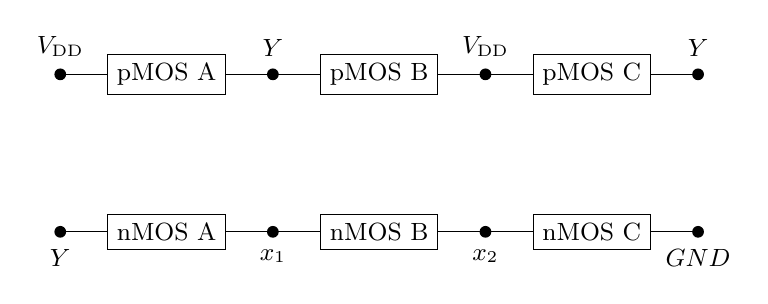
\begin{tikzpicture}[x=1.35cm,y=1cm,font=\small]
\foreach \x/\lab in {0/{V_{\mathrm{DD}}},2/Y,4/{V_{\mathrm{DD}}},6/Y} {
\node[circle,fill,inner sep=1.5pt] at (\x,2) {};
\node[above] at (\x,2.1) {$\lab$};}
\foreach \x/\lab in {1/A,3/B,5/C} {
\draw (\x-1,2)--(\x+1,2) node[midway,draw,fill=white] {pMOS \lab};}
\foreach \x/\lab in {0/Y,2/{x_1},4/{x_2},6/{GND}} {
\node[circle,fill,inner sep=1.5pt] at (\x,0) {};
\node[below] at (\x,-0.1) {$\lab$};}
\foreach \x/\lab in {1/A,3/B,5/C} {
\draw (\x-1,0)--(\x+1,0) node[midway,draw,fill=white] {nMOS \lab};}
\end{tikzpicture}
\end{latin}
\caption{نمای اتصال ناحیه‌های متوالی \lr{Diffusion} در \lr{NAND} سه‌ورودی.
این شکل نمودار اتصال است، نه شماتیک ابعادی: گره‌های هم‌نام بالا با فلز مشترک
می‌شوند؛ دو گره داخلی پایین مستقل‌اند. بلوک‌ها کانال‌های کنترل‌شده‌اند و سیم ثابت نیستند.}
\label{fig:layout-nand-chain}
\end{figure}

شکل \ref{fig:layout-nand-stick} همین اتصال‌ها را در نمای لایه‌ای نشان می‌دهد.
ابتدا فقط نوارهای \lr{Diffusion} و سه خط \lr{Poly} را بخوانید؛
سپس بررسی کنید هر تماس با کدام سیم فلزی به ریل یا خروجی وصل شده است.
\begin{figure}[ht]
\centering
\begin{latin}
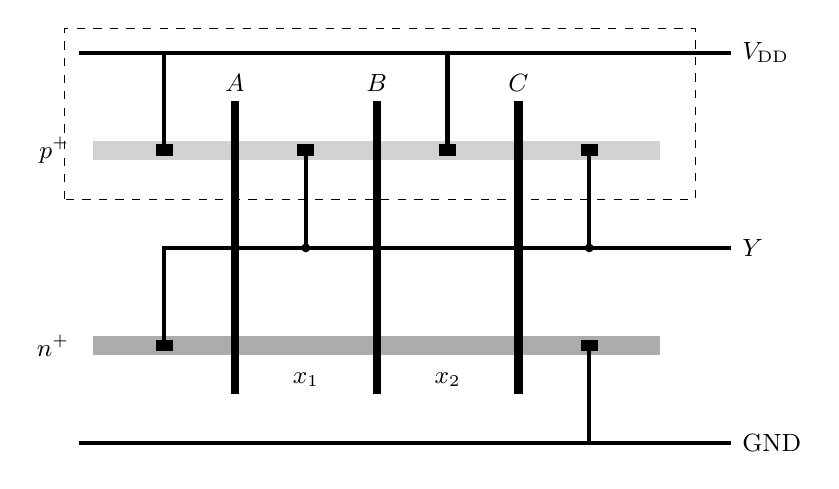
\begin{tikzpicture}[x=0.9cm,y=0.62cm,font=\small]
\draw[dashed] (-0.4,5) rectangle (8.5,8.5);
\draw[line width=7pt,gray!35] (0,6)--(8,6);
\draw[line width=7pt,gray!65] (0,2)--(8,2);
\node[left] at (-0.2,6) {$p^+$};\node[left] at (-0.2,2) {$n^+$};
\foreach \x/\lab in {2/A,4/B,6/C} {
\draw[line width=3pt] (\x,1)--(\x,7);
\node[above] at (\x,7) {$\lab$};}
\draw[line width=1.5pt] (-0.2,8)--(9,8) node[right] {$V_{\mathrm{DD}}$};
\draw[line width=1.5pt] (-0.2,0)--(9,0) node[right] {GND};
\draw[line width=1.5pt] (1,6)--(1,8) (5,6)--(5,8);
\draw[line width=1.5pt] (3,6)--(3,4) (7,6)--(7,4);
\draw[line width=1.5pt] (1,2)--(1,4)--(9,4) node[right] {$Y$};
\draw[line width=1.5pt] (7,2)--(7,0);
\foreach \x/\y in {1/6,3/6,5/6,7/6,1/2,7/2} {
\fill (\x-0.12,\y-0.12) rectangle (\x+0.12,\y+0.12);}
\foreach \x in {3,7} {\fill (\x,4) circle (1.6pt);}
\node at (3,1.3) {$x_1$};\node at (5,1.3) {$x_2$};
\end{tikzpicture}
\end{latin}
\caption{\lr{Stick Diagram} آموزشی \lr{NAND} سه‌ورودی بر پایه شکل‌های
\secnum{۱.۴۲} و \secnum{۱.۴۳} کتاب \cite{weste}.
خط‌های عمودی ضخیم \lr{Poly} و خطوط نازک سیاه \lr{Metal1} هستند؛
تقاطع آن‌ها در مسیر افقی \(Y\) بدون تماس است.
مربع‌ها تماس فلز با \lr{Diffusion} و نقطه‌های گرد اتصال فلز با فلزند.
تماس‌های بدنه برای خلوت ماندن شکل حذف شده‌اند و باید در \lr{Layout} نهایی اضافه شوند؛
اندازه‌های شکل مطابق قواعد رسم نشده‌اند.}
\label{fig:layout-nand-stick}
\end{figure}

در ورودی \((A,B,C)=(1,1,1)\)، سه کانال پایین هدایت دارند و خروجی به زمین می‌رسد؛
هر سه \lr{pMOS} قطع‌اند. اگر مثلاً \(B=0\)، کانال میانی پایین قطع و
\lr{pMOS} مربوط به \(B\) روشن است؛ چون دو سر آن با فلز به خروجی و تغذیه
وصل‌اند، خروجی یک می‌شود. این استدلال برای صفر بودن \(A\) یا \(C\) نیز برقرار است.

اشتراک ناحیه می‌تواند تماس، سیم و مساحت را کم کند؛ هندسه آن بر ظرفیت
\lr{Diffusion} هم اثر می‌گذارد. بااین‌حال، نمی‌توان هر دو ناحیه دلخواه را
ادغام کرد؛ نوع ماده، چاه و شبکه الکتریکی باید سازگار باشند.
یکسان بودن ظاهر خط \lr{Diffusion} به معنی یکسان بودن همه گره‌های آن در حضور
\lr{Gate}های قطع‌کننده مسیر نیست.

\subsection{ریل‌ها، کنارهم‌گذاری سلول و دسترسی پایه}
در سبک کتاب، ریل‌های فلزی بالا و پایین تا مرز سلول ادامه دارند.
فاصله مرزی باید طوری باشد که کنارهم‌گذاری دو سلول نیز قواعد را حفظ کند؛
کتاب در مثال، بیرون‌زدگی \(2\lambda\) ریل در هر طرف را برای تامین فاصله
\(4\lambda\) محتوای دو سلول توضیح می‌دهد.
این عدد به هندسه همان شکل وابسته است، نه قاعده عمومی همه مرزهای سلول
\cite[صفحه چاپی ۲۷]{weste}.

دسترسی به پایه فقط نام‌گذاری آن نیست؛ باید مسیر و فضای اتصال برای سیم‌کشی
سلول‌های دیگر وجود داشته باشد. مثال ساده کتاب اجازه دسترسی \lr{Poly} از بالا
یا پایین را می‌دهد؛ ادامه متن توضیح می‌دهد که دسترسی فلزی و تماس‌های
\lr{Metal2--Metal1--Poly} در سبک‌های دیگر می‌تواند فضای بیشتری لازم داشته باشد.
پس کوچک‌ترین نقشه داخلی، الزاماً بهترین سلول قابل مسیریابی نیست.

\section{\lr{Stick Diagram} و برآورد مساحت}
\label{sec:layout-stick}
\subsection{چه چیزی را حفظ و چه چیزی را حذف می‌کنیم؟}
\lr{Stick Diagram} نمایش سریع توپولوژی لایه‌ها و اتصال‌هاست؛
خط‌ها لازم نیست عرض یا فاصله واقعی داشته باشند.
نوع لایه، محل ترانزیستور و تماس و ترتیب اتصال‌ها حفظ می‌شود؛
اما جزئیات مستطیل‌ها و اندازه‌گذاری نهایی به \lr{Layout} واگذار می‌شود
\cite[بخش \secnum{۱.۵.۵}]{weste}.
بنابراین شکل \ref{fig:layout-inverter} از نظر نقش آموزشی به یک \lr{Stick Diagram}
نزدیک است؛ مرز تماس‌ها و چاه فقط برای فهم بهتر اضافه شده‌اند.
صرف کشیدن یک طرح باریک، مساحت کمتر قابل ساخت را اثبات نمی‌کند.

\subsection{از \lr{Routing Track} به ابعاد تقریبی}
یک \lr{Routing Track} فضایی برای یک سیم و فاصله لازم تا سیم مجاور است.
برای عرض فلز \(4\lambda\) و فاصله آزاد \(4\lambda\)،
\lr{Track Pitch} برابر \(8\lambda\) می‌شود.
اگر \(N_x\) و \(N_y\) تعداد بازه‌های ترک در دو جهت باشند، تخمین اولیه این است:
\begin{equation}\label{eq:layout-area}
W_{\mathrm{cell}}\approx8\lambda N_x,\qquad
H_{\mathrm{cell}}\approx8\lambda N_y,\qquad
A_{\mathrm{cell}}\approx64N_xN_y\lambda^2.
\end{equation}
در رابطه سوم، دو طول را ضرب کردیم؛ پس واحد مساحت \(\lambda^2\) است، نه
\(\lambda\). این تقریب به سبک و قواعد همان مدل متکی است.
شمارش \lr{Track} به معنی شمردن تعداد ترانزیستور یا صرفاً تعداد خط‌های مرئی نیست؛
فضاهای لازم و حاشیه‌ها هم سهم دارند.

مرز چاه باید از \lr{pMOS} به اندازه \(6\lambda\) فاصله پوشش داشته باشد
و از \lr{nMOS} نیز \(6\lambda\) دور باشد. بنابراین در این مدل،
میان دو ناحیه ترانزیستوری حداقل فضای \(12\lambda\) لازم می‌شود.
کتاب اثر این فاصله را با اختصاص یک \lr{Track} اضافی میان دو ردیف لحاظ می‌کند؛
حتی اگر آن ترک واقعاً سیمی نداشته باشد
\cite[شکل‌های \secnum{۱.۴۴} و \secnum{۱.۴۵}]{weste}.
نباید \(12\lambda\) را با فاصله آزاد معمول فلز \(4\lambda\) یکی گرفت.

\subsection{مثال کتاب: مساحت \lr{NAND} سه‌ورودی}
در شکل \secnum{۱.۴۶} کتاب، چهار ترک در جهت عرض و پنج ترک در جهت ارتفاع
شمارش شده‌اند. بنابراین:
\begin{equation*}
W_{\mathrm{cell}}\approx32\lambda,\qquad
H_{\mathrm{cell}}\approx40\lambda,\qquad
A_{\mathrm{cell}}\approx1280\lambda^2.
\end{equation*}
کتاب ارتفاع بدنه سلول را \(36\lambda\) و ارتفاع با فضای اضافی
\(4\lambda\) مجاور را \(40\lambda\) معرفی می‌کند؛
اختلاف این دو عدد ناشی از تعریف مرز شمارش مساحت است
\cite[صفحات چاپی ۲۷ تا ۲۹]{weste}.
هنگام مقایسه دو مساحت باید معلوم باشد فاصله بین سلول‌ها نیز شمرده شده است یا نه.

با انتخاب آموزشی \(\lambda=\qty{0.3}{\micro\metre}\)، ابعاد و مساحت می‌شوند:
\begin{align*}
W_{\mathrm{cell}}&\approx\qty{9.6}{\micro\metre},&
H_{\mathrm{cell}}&\approx\qty{12}{\micro\metre},\\
A_{\mathrm{cell}}&\approx1280(0.3)^2\,\unit{\square\micro\metre}
=\qty{115.2}{\square\micro\metre}.
\end{align*}
ضریب \(0.3\) باید به توان دو برسد؛ زیرا تبدیل واحد مساحت از ضرب دو طول می‌آید.
این عدد، برآورد هندسی با ورودی‌های فرض‌شده است و گزارش اندازه‌گیری یک تراشه نیست.

\subsection{مثال کتاب: گیت \lr{OAI31}}
تابع مثال \secnum{۱.۳} کتاب،
\(Y=\overline{(A+B+C)D}\) است؛ مکمل روی کل عبارت قرار دارد.
پایین، گروه موازی \(A,B,C\) با \(D\) سری و بالا، گروه سری \(A,B,C\)
با \(D\) موازی می‌شود.
برای شکل \secnum{۱.۴۷}، کتاب پنج و شش ترک را در دو جهت گزارش می‌کند،
پس ابعاد تخمینی \(40\lambda\times48\lambda\) و مساحت
\(1920\lambda^2\) است \cite[صفحه چاپی ۲۹]{weste}.
این تخمین برای همان ترتیب و مسیرهای شکل است؛ بهینه بودن آن برای هر فرایند اثبات نشده است.

با مقیاس مثال قبلی، ابعاد \(\qty{12}{\micro\metre}\) و
\(\qty{14.4}{\micro\metre}\) و مساحت
\(\qty{172.8}{\square\micro\metre}\) می‌شود.
نسبت مساحت به \lr{NAND} قبلی برابر \(1920/1280=1.5\) است؛
این نسبت برای دو برآورد با قواعد و مرز یکسان معتبر است.

\subsection{چرا این برآورد محدود است؟}
اگر عرض ترانزیستور از \(4\lambda\) بیشتر شود، فضای اضافه آن باید لحاظ شود.
تعداد و محل تماس‌ها، دسترسی پایه، لایه فلزی، مرز چاه و سیم‌کشی نیز
می‌توانند تعداد ترک لازم را تغییر دهند.
پس رابطه \eqref{eq:layout-area} نقشه راه اولیه است، نه جانشین طراحی دقیق
و کنترل قواعد کامل. کتاب نیز برای سلول‌های حساس، ساخت آزمایشی \lr{Layout}
را لازم می‌داند \cite[ابتدای صفحه چاپی ۲۹]{weste}.

\section{تمرین‌های جمع‌بندی و پاسخ تشریحی}
\subsection{پرسش‌ها}
\begin{enumerate}
\item اگر یک خط فلز از روی \lr{Poly} عبور کند و تماس نداشته باشد، آیا دو شبکه متصل‌اند؟
\item چرا در نوار \lr{p-diffusion} گیت \lr{NAND}، سیم‌کشی همه گره‌ها به یک فلز مشترک غلط است؟
\item برای \(\lambda=\qty{0.1}{\micro\metre}\)، عرض \(4\lambda\)،
تماس \(2\lambda\) و مساحت \(1280\lambda^2\) را به واحد فیزیکی تبدیل کنید.
\item سه خط \lr{Metal1} به عرض \(4\lambda\)، با دو فاصله آزاد
\(4\lambda\)، مجموعاً چه پهنایی اشغال می‌کنند؟ فاصله مرکز خط اول تا سوم چقدر است؟
\item اگر در همان مدل تخمین، مقیاس \(\lambda\) نصف شود، طول‌ها و مساحت چه تغییری می‌کنند؟
آیا این نتیجه امکان انتقال مستقیم نقشه به هر فرایند دیگری را ثابت می‌کند؟
\end{enumerate}

\subsection{پاسخ‌ها و کنترل نتیجه}
\begin{enumerate}
\item در مدل لایه‌های عایق‌شده خیر؛ برای اتصال \lr{Metal1} به \lr{Poly}
تماس مناسب لازم است. در مقابل، عبور \lr{Poly} از \lr{Active} نقش ترانزیستوری دارد.
\item همه گره‌های میان کانال‌ها نباید یک شبکه باشند؛ با اتصال همگی به یک فلز،
دو ریل یا پایانه‌های لازم کوتاه می‌شوند و نقش ترانزیستورها از بین می‌رود.
در مثال، گره‌های متوالی باید به‌تناوب تغذیه و خروجی باشند.
\item عرض \(\qty{0.4}{\micro\metre}\)، ضلع تماس
\(\qty{0.2}{\micro\metre}\) و مساحت
\(1280(0.1)^2=\qty{12.8}{\square\micro\metre}\) است.
\item پهنای لبه بیرونی تا لبه بیرونی برابر
\((3\times4+2\times4)\lambda=20\lambda\) است.
فاصله مرکز اول تا سوم دو \lr{Pitch}، یعنی \(16\lambda\) است؛
این دو اندازه یکسان نیستند. برای \(n\) خط هم‌اندازه، پهنای فیزیکی
\(nw+(n-1)s\) و فاصله دو مرکز انتهایی \((n-1)(w+s)\) خواهد بود.
\item در مدل تشابه هندسی، هر طول نصف و مساحت یک‌چهارم می‌شود.
اما قواعد واقعی ممکن است یکسان مقیاس نشوند؛ پس قابلیت ساخت در فرایند دیگر
از این محاسبه نتیجه نمی‌شود.
\end{enumerate}

\subsection{روش بازبینی یک طرح تازه}
ابتدا تعداد تقاطع‌های \lr{Poly/Active} را با تعداد ترانزیستورهای شماتیک مقایسه کنید.
سپس هر ناحیه \lr{Diffusion}، فلز و تماس را به یک شبکه نام‌گذاری‌شده نسبت دهید.
نوع ترانزیستور و اتصال بدنه را کنترل کنید؛ در پایان ابعاد، فاصله‌ها و دسترسی پایه‌ها را بررسی کنید.
این ترتیب، خطای اتصال را از خطای هندسی جدا می‌کند.

در ابزارهای طراحی، \lr{DRC} قواعد هندسی و \lr{LVS} تطبیق مدار استخراج‌شده با
شماتیک را بررسی می‌کنند؛ عبور از یکی به معنی عبور از دیگری نیست.
در این جزوه کنترل‌های آموزشی محاسبه و توپولوژی انجام می‌شوند؛
تایید صنعتی به فایل‌های فرایند و ابزارهای مربوط نیاز دارد.
با این پایه، می‌توان در ادامه فصل از طراحی یک سلول به سازمان‌دهی یک مدار بزرگ‌تر رسید.

\begin{thebibliography}{9}
\bibitem{weste}
\begin{latin}
Neil H. E. Weste and David Money Harris,
\textit{CMOS VLSI Design: A Circuits and Systems Perspective},
Fourth Edition, Pearson, 2011.
\end{latin}
بخش \secnum{۱.۵}: صفحات چاپی ۱۹ تا ابتدای ۲۹؛ صفحات ۴۶ تا ۵۶ فایل \lr{PDF}.
مقطع و مجموعه ماسک: شکل‌های \secnum{۱.۳۴} و \secnum{۱.۳۵}؛
مراحل ساخت: \secnum{۱.۳۶} تا \secnum{۱.۳۸}؛ قواعد و ابعاد:
\secnum{۱.۳۹} و \secnum{۱.۴۰}؛ گیت‌ها و تخمین مساحت:
\secnum{۱.۴۱} تا \secnum{۱.۴۷}.
شکل‌های این جزوه بازترسیم آموزشی و دارای شماره داخلی مستقل‌اند.
\bibitem{intro}
اسلایدهای محلی \lr{Introduction}، فایل \lr{00-introduction.pdf}،
اسلایدهای ۲۱ تا ۲۷، درباره مدل \lr{Switch} و گیت‌ها.
طبق اسلاید ۲، یادداشت‌های اصلی متعلق به \lr{David Money Harris}، سال ۲۰۱۱،
و نسخه محلی اقتباس‌شده است.
\bibitem{mos}
اسلایدهای محلی \lr{MOSFET Transistors}، فایل \lr{01-MOSFET Ch2.pdf}،
اسلایدهای ۵ تا ۷ برای ساختار مقدماتی؛ اسلایدهای ۱۵ و ۲۴ برای
جهت‌های \(W,L\) و ارتباط هندسه با ظرفیت.
در فایل‌های اسلاید، شماره صفحه و شماره اسلاید یکسان است.
\end{thebibliography}
\end{document}
